\section{Algorithm}
\label{sec:algo}
The core recommendation engine consists of two modules:
the offline web information extraction module and the online
user model and recommendation model. The first module is responsible
for collecting in advance weekly TV listing of all the cable channels in China,
identifying the program titles and show times, and then extracting relevant
information about the programming from the web. All of these are
considered preprocessing before the actually real-time recommendation
begins. The second module maintains the user viewing model dynamically
and by comparing the similarity between the current user model and the future
programs, recommends the most relevant programs to the user in real time.
We next present these two modules in detail.
%
%\subsection{Web Information Extraction}
%\begin{itemize}
%\item Preprocessing of TV listing
%
%\item Extraction of Show Information
%  \begin{enumerate}
%	\item Program synopsis
%	\item Program meta data
%  \end{enumerate}
%\end{itemize}

\subsection{Viewer Model and Recommendation}
%\begin{itemize}
%\item Vector model for a TV program
%\item Viewer model = viewed programs + preference weights
%\item Similarity measures and recommendation
%\end{itemize}

Our TV program recommendation system will first get program information from the Internet according to the program schedule. We simply put the program name on search engines like  Google and Baidu, then we will get many related links towards the information we might need. However, the websites these links lead to may contain many noises. In order to filter noises while extracting the main content, we have developed a simple but nice web information filter. It will delete almost all the ads and keep the main content untouched.

In order to analyze a web page for content extraction, we first pass web pages through an HTML parser that will correct wrong markups and construct a Document Object Model(DOM) tree.
%Figure \ref{fig:dom}
%is an example. With the help of DOM tree, we can navigate the HTML file with ease and extract content more precisely.
%\begin{figure}
%\begin{center}
%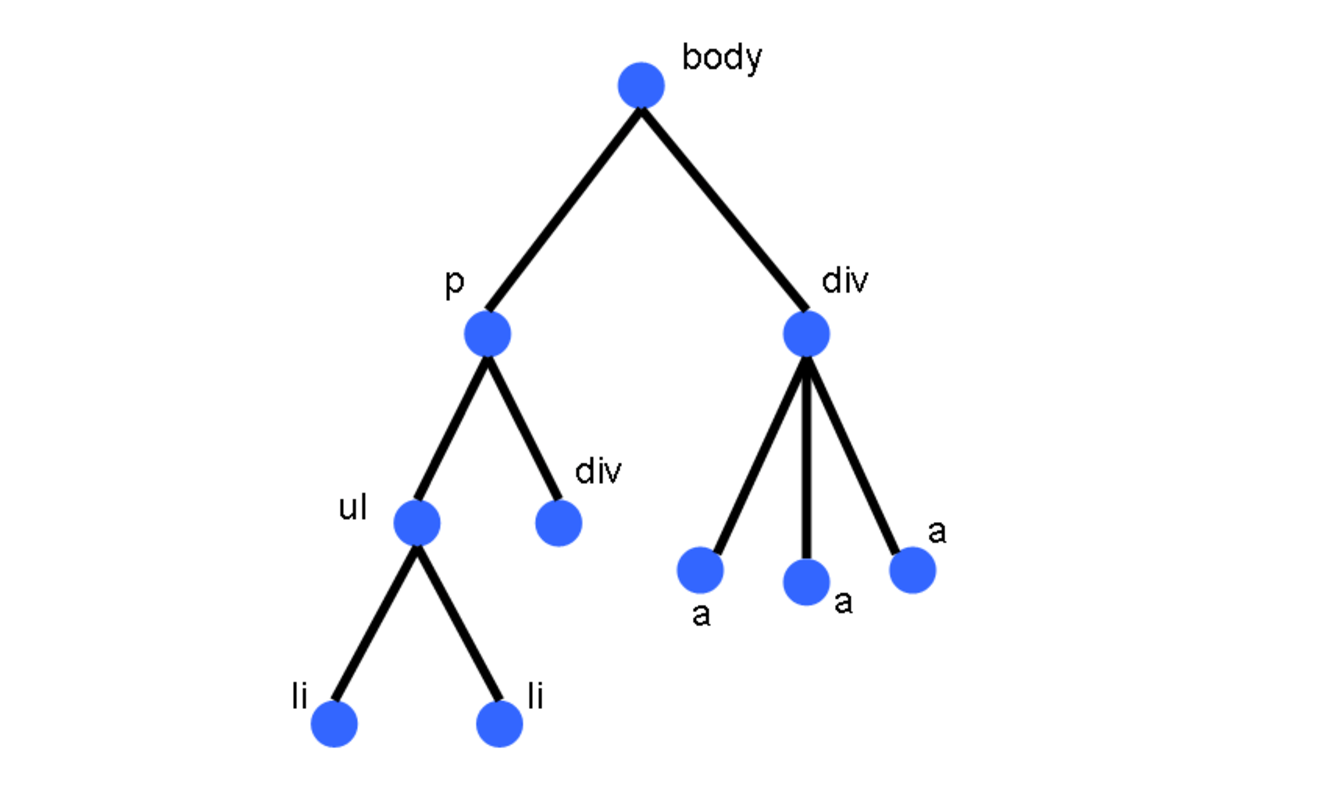
\epsfig{file=domtree.eps,width=\columnwidth}
%\caption{\label{fig:dom}DOM Tree Analysis}
%\end{center}
%\end{figure}

Our web information filter is based on the following observations:
\begin{itemize}
\item The main content of a web site is likely to be displayed together.
\item Ads and other noises are likely to be links.
\item Different data are often divided by certain tags like $<p>$, $<div>$, $<table>$, etc.
\end{itemize}
Based on these observations, we develop a criterion, that is, if the proportion of the link texts in a certain block divided by $<p>, <div>, <table>$, etc is greater than a threshold, then this block is classified into noises and therefore deleted, otherwise it is kept. This idea seems to be quite simple, but with several DOM tree navigation methods it works quite well.
According to the third observation, we should analyze the HTML files block by block. Yet there may be blocks nested into each other. We employed postorder traversal of the DOM tree. In that way, the most nested block will be classified first, then we move on to the other blocks. Once a block is classified, it will be sent upward whether it is content or noise, which will help to judge the outside nest block.

In the DOM tree, each HTML tag is presented as a node. When we traverse the tree in postorder, if we meet a tag that is by no means the main text content, i.e, $<img>, <script>$, this node and its children are removed from the tree. We can maintain a blacklist which contains all these ill tags that should be deleted immediately once met. If the node is not on the blacklist and it is not a block tag, then we put it into the candidate list. If the node is a block tag, then it can be judged by the criterion above with all the candidates taken into consideration. In a nested block, the outside block contains offsprings that are also blocks and have already been judged in the postorder traversal. If the offspring is noise, then it has been removed and has no impact on our later judgement. If it is kept, then in our later judgement, the links and texts in it should also be calculated in the criterion.

The navigation stops when we meet the $<body>$ tag. The filtering is over and the main content is extracted.

Once we get the TV program information from the Internet, segmenter is then involved to segment the documents into terms. Chinese language is quite different from English. In Chinese, segmentation is of more importance than stemming and lemmatization. Once a document is correctly segmented, we can say that we have get the main idea of it. Here, We employ ICTCLAS, a worldwide famous tool in the field of natural language understanding, to do the job. Meanwhile, stop words are taken into consideration to avoid valueless matches.

At the same time, we construct the inverted index.
Inverted index is a basic data structure in information retrieval system.
We employ it here for the sake of fast retrieval and nice representation of document bag model. After we have done the tokenization job, we try to construct the inverted index with sort-based indexing method. Every posting list's head is a term, and then there is a table that contains all the document ids where this term appears. There are many other data stored in the inverted index, too, like term frequency, document frequency, etc.
%\begin{figure}
%\begin{center}
%\epsfig{file=index.eps,width=\columnwidth}
%\caption{\label{fig:index}Inverted Index}
%\end{center}
%\end{figure}
In our system, we not only consider whether a term appears in a document but also how frequently it appears. It is called term frequency, and it is determined by the times a term appears in the document. But the original term frequency suffers a serious problem, that is, it treats every term with the same importance. But we can easily see that some terms have none or few ability to tell documents apart. And then naturally, we turn to term frequency-inverse document frequency(tf-idf):
\begin{equation}
tf-idf=\log(tf+1)\times\log(N/df)
\end{equation}
In the equation above, tf is the term frequency in one document, N is the total number of the document and df is the number of the documents that contain the term. In other word, tf-idf assigns weights to a term denoted by t in the following ways:
\begin{itemize}
\item If t appears many times in a small number of documents, it gets the highest weight since it is very powerful to tell these documents apart.
\item If t rarely appears in one document, or it appears in many documents, it enjoys median weight.
\item If t appears in all documents, it gets the lowest weight.
\end{itemize}
It can be immediately seen that if one thinks involving stop words a tiring job, then tf-idf may help ease the pain because stop words are likely to appear in almost all the documents, then they will get the lowest weights.

For a certain document, the compressed term set version got from the tf-idf calculation can be treated as another representation of the document. It is called bag of words model in the field of information retrieval. Only frequency is considered in this model, not the order terms appear, yet we still think it to be close to the original document.

Based on the bag of words model, we construct the vector space where every dimension represents the relative importance of a term in the document. Suppose the vector of a document is denoted as V(d),  every dimension of which is corresponding to a term. And the weight of every dimension is calculated by tf-idf. Then the similarity of two document is calculated by cosine similarity:
%(see Figure
%\ref{fig:similar}):
%\begin{figure}
%\begin{center}
%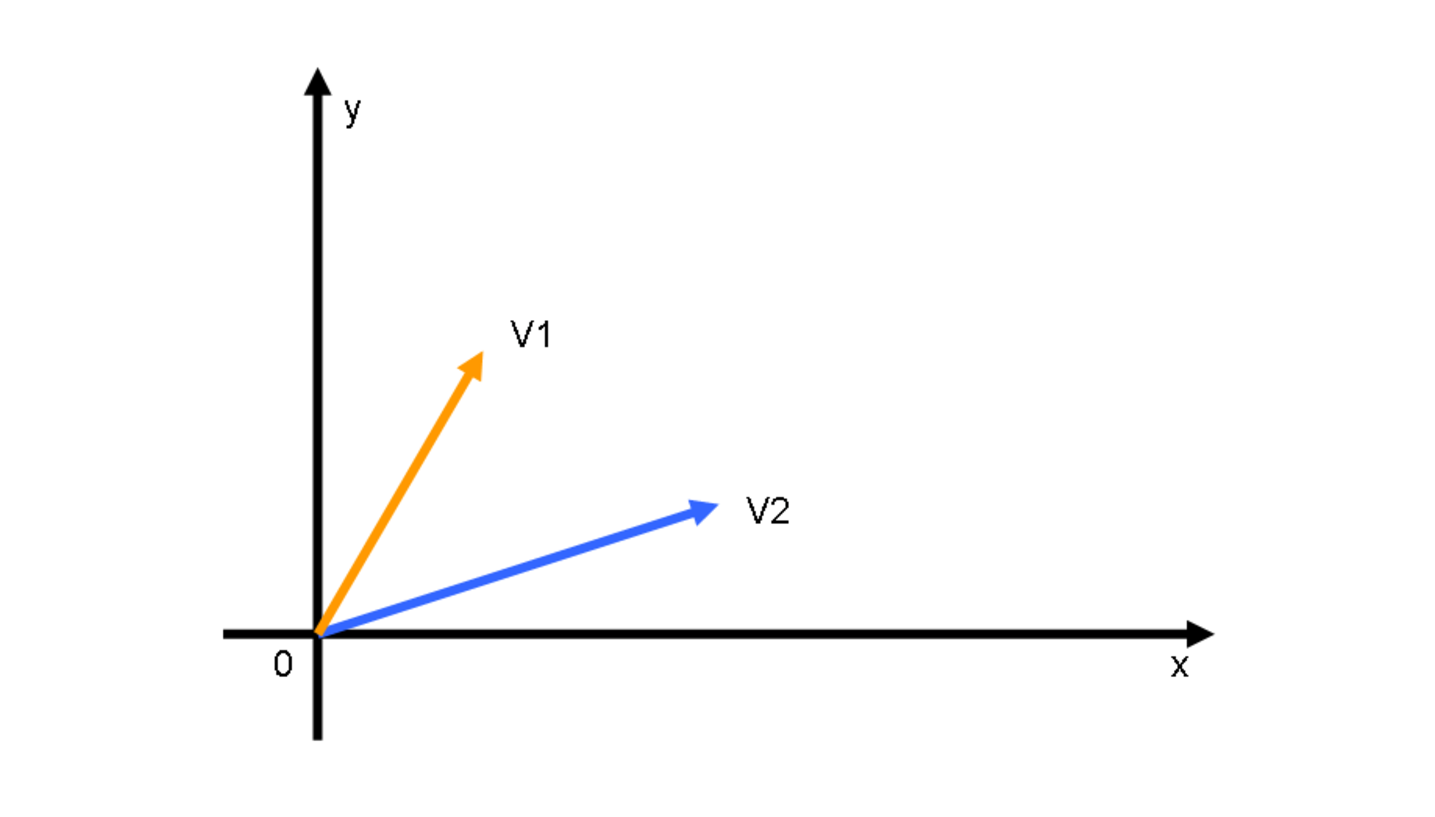
\epsfig{file=similar.eps,width=\columnwidth}
%\caption{\label{fig:similar}Program Vector Combination}
%\end{center}
%\end{figure}
\begin{equation}
sim(d1,d2)=\frac{V(d1)\bullet V(d2)}{|V(d1)|\times|V(d2)|}
\end{equation}
Naturally, to represent a collection of documents as a set of vectors is the same as to convert the whole document collection into an M*N term-document matrix where M is the number of terms and N is the number of documents. We will see the use of it later.

Since the search engine may return several links for one TV program, there will be several documents describing the same program.
Therefore, we combine them together to produce one vector space for each TV program in the same way(see Figure \ref{fig:vector}).

\begin{figure}
\begin{center}
\epsfig{file=programvector.eps,width=\columnwidth}
\caption{\label{fig:vector}Synopsis Vector Combination}
\end{center}
\end{figure}

So far the whole vector space of TV programs is constructed. We convert the vector space into a P*Q matrix where the P is the number of terms and Q is the number of TV programs. And then we employ Latent Semantic Analysis(LSA).

In Chinese language, one word or term may mean different meanings in different circumstances while the same meaning may be expressed in different words. This characteristic causes severe problems in our analysis of the document bag model. Meanwhile, as the document number increases, the number of terms also increases, which result in high dimensions in the vector space and time-consuming calculation of the vector. In order to reduce the dimension while reduce the influence of the two typical characteristics stated above, LSA is a good choice.

Deerwester(1990) combined the work of matrix low-rank approximation with IR. We do not go deeper into LSA but give a simple outline about it. The mathematic foundation is matrix decomposition: singular value decomposition(SVD). Suppose a matrix C is decomposed into C=USV, where S is the diagonal matrix of singular values. Then we eliminate several smallest singular values of S, and recalculate the new C with the new S. Generally speaking, the matrix low-rank approximation is a constrained optimization problem. We denote the new C as M, then we recalculate the similarity matrix R=M'M. The (i,j) unit of R is the similarity between program i and j. We can see that when the dimension is reduced, SVD will combine the terms that tend to appear together. Thus the similarity precision will not decline much, but increase sometimes.

A good recommendation system must classify the products into several categories. Our system will classify the TV programs according to the descriptions extracted from the Internet, which means it is similar to the document classification. We observe that the more similar two programs are, the closer the two vectors of the two programs are. In general, document classification may be divided into two categories: unsupervised and supervised. Supervised methods include k nearest neighbor(kNN), Rocchio, etc. Unsupervised methods include flat clustering, hierarchical clustering, etc. Here we employ single-link clustering method, quite simple but enough for our application. Single-link clustering is a hierarchical clustering. We first consider every program as a cluster, and then keep doing combining job, or say agglomerating job, until all the programs are in one cluster. The procedure we do clustering will yield a dendrogram, which will help to do the recommendation as we'll see later. The advantage of clustering is that the number of clusters don't need to be set in advance. The only thing we need to do is set a threshold or criterion to judge whether we should stop and get several groups with no intersections. Single-link clustering and complete-link clustering are quite similar except the calculation of the distance between two cluster. Single-link defines the distance as the similarity between two most alike member of the two cluster while complete-link uses the two most unlike members. As we state above, the description about programs is from the Internet, there will be noises involved. Complete-link pays too much attention to the noises, which might cause some problems. So we use single-link clustering in our system. Chaining is a typical problem in single-link. But we are designing a recommendation system, so the chain cluster can also work because the inner similarity still exists. In the other aspect, the probability of chaining is quite small considering the high variation of documents extracted from the Internet.

The above is the design of the off-line system. We now explain the interface to the client.

For each client, there is a vector corresponding to his or her preference. Note that each dimension now is not a term but the dimension we've derived using LSA. Thus the dimension is relatively low. It will help to increase the efficiency.

When the client turns on the TV, he may switch between different channels. We capture his or her action, analyzing his or her preference. The simplest way is to store how long he or she has seen a program, and use that to judge whether he or she likes it or not. Different length, different weight of how he or she likes the program. When we can judge a client likes a program, we combine the vector of the program into his or her vector with appropriate weight. Then the vector describes the client's preferences. If the client's vector is similar to a program's vector, we may say he or she likes the program. In order to recommend more programs that clients may like, the cluster we get using single-link clustering now plays a main role. If the vector of the client is similar to the vector of a program, then we not only recommend that specific program, but also all the  programs of the cluster that program belongs to.

In order to find the nearest neighbor of the client's vector denoted as V, we can use the dendrogram we get as by-product when we do the clustering. We search form the root of the tree, then calculate the similarities of V against the two children node(it can be easily proved that every node can only have two or none children in the dendrogram). Then we choose the closest child and go down and down until we reach the leaf node or meet a certain threshold, i.e, we must return a certain number of programs. In this way, the simplest recommendation is achieved.

The vital difference between TV programs recommendation system and other system lies in that programs are highly time varying. That means, time factor should also be taken into consideration. For example, one client only watches TV at night and he must go to work at day. Then it doesn't make any sense to recommend programs that only show at day. One simple way to deal with this problem is to filter all the programs the recommendation system has returned to remove all the wrong-time program. This idea might work, but might remove all the programs just because of the time. We employ another way to deal with the problem, considering both the time and program similarities.
\begin{figure}
\begin{center}
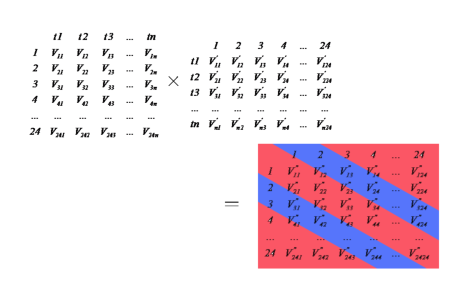
\epsfig{file=matrix.eps,width=\columnwidth}
\caption{\label{fig:matrix}Time Variation Matrix}
\end{center}
\end{figure}
Each program may be aired at different time of a day. We can divide the day into several periods, like into 24 segments indicating 24 hours of a day. Then we expand the vector of the program into an M*N matrix where M is the number of time periods and N is the LSA dimension. If the program is aired in time period i and j, the the i row and the j row will both be filled with the LSA vector we get before. The similarity of two matrices A and B is defined as:
Calculate R=A*B'. Figure \ref{fig:matrix} shows an example. R is an M*M matrix, indicating how similar two programs are in every period. It can be seen that on the diagonal the result shows the similarity of two programs on the same time. Of course, if they are not aired the same time, the number will be zero. Then we can see that the nearest the unit of R is to the middle of diagonal and the corner(red color part in Figure \ref{fig:matrix}), the irrelevant two programs may be because of the time difference. Based on this observation, we may develop a function to describe this decaying weight. Then we summarize all the products of unit value and decaying weight, and draw the final similarity value.

Clients' vectors can be expanded into matrices and calculated the same way. We do not explain in detail again.

\subsection{Discussions}
After some analysis, we find that the content-based method cannot cover
all the programs. The content-based method does do well in some kinds
of programs like movie and drama, because it's easy to get detailed
description and abstract of them from the Internet.
But for programs like news and talk shows, the information from the
Internet is not enough to characterize them. In
this case, we consider to use meta data as supplement. We first form a standard meta data
structure. Basically it contains some attribute-value pairs. When we need to get the meta data
structure of one program, we just combine the program name and attribute name together as the
key word then search the Internet. In the HTML files we receive, we check if the attribute
name appears in text pairs. If so, its partner will be seen as the value. Similar to the vector
method, we can use meta data structure to describe a program, we can use the structures of all
the programs user has viewed to form a user meta data structure, then we can process similarity
comparison between these two kinds of structure.

Here we point out two kinds of function, $C_u$(p) and $M_u$(p). $C_u$(p) is defined as the
similarity between user vector and program vector. $M_u$(p) is defined as the similarity
between user meta data structure and program meta data structure. In order to merge this
two results, we define the equation below:

\[P_u(p) = \alpha(C_u(p))+\beta(M_u(p))\]

$\alpha$ and $\beta$ are two functions that will be decided by nonlinear fitting method.

Follow this idea, we provide an equation to calculate the similarity between users and programs:

\[P_u(p) = \sum_{i=1}^nw_i\delta(v_{u_i},v_{p_i})\]

In this equation, we simply $\alpha$ and $\beta$ as linear function and combine vector generated
from synopsis and meta data together to form a general attribute structure.

$\delta(v_{u_i},v_{p_i})$ is used to calculate for each attribute in the attribute structure,
the similarity between value of users and value of programs. Take into account the different
type of attributes, we design three different implementations of this function.

\begin{itemize}
\item synopsis
\item time
\item meta data
\end{itemize}

For synopsis, since it is constructed as vector, we simply calculate the cosine value between
two synopsis vector and take it as the similarity.

For time, since its value is a range, we can calculate the intersection and union of two time
range. Then divide the length of intersection by the length of union and use the ratio as
the similarity.

For meta data, the value of an attribute is actually a set. Similar to how we deal with time,
we calculate the intersection and union of two value sets, divide the size of intersection by
the size of union then use the result as the ratio as the similarity.

In our equation, each attribute similarity has a weight parameter $w_i$. Our concern is that
for different users, the effect that one attribute influence their choice is different. $w_i$ is
used to define the importance of one attribute to users. $w_i$ is unknown at first, but we
can learn it based on users' behaviour.




















